

%\usepackage{scicite}

%\usepackage{times}
%\usepackage{graphicx}
%\usepackage{verbatim}
%\usepackage{subfigure}
%\usepackage{tikz}
%\usepackage{amsmath}
%\usepackage{amssymb}
%\usepackage{array}
%\usepackage{tabularx}
%\usepackage{multirow}
%\usepackage{multicol}
%\usepackage{multibox}
%\usepackage{rotating}
%\usepackage{color}
%\usepackage{layout}
%\usepackage{epstopdf}
%\usepackage{afterpage}
%\usepackage[left]{lineno}

%% PNAStmpl.tex
%% Template file to use for PNAS articles prepared in LaTeX
%% Version: Apr 14, 2008


%%%%%%%%%%%%%%%%%%%%%%%%%%%%%%
%% BASIC CLASS FILE 

\documentclass{pnastwo}

%%%%%%%%%%%%%%%%%%%%%%%%%%%%%%
%% OPTIONAL GRAPHICS STYLE FILE

\usepackage[pdftex]{graphicx}

%%%%%%%%%%%%%%%%%%%%%%%%%%%%%%
%% OPTIONAL POSTSCRIPT FONT FILES

\usepackage{pnastwof}

%%%%%%%%%%%%%%%%%%%%%%%%%%%%%%
%% ADDITIONAL OPTIONAL STYLE FILES

\usepackage{amssymb,amsfonts,amsmath}
\usepackage[font=large]{caption}
\usepackage{subfigure}
\usepackage{epstopdf}
\usepackage{graphicx}
\usepackage{verbatim}
\usepackage{array}
\usepackage{tabularx}
\usepackage{multirow}
%\usepackage{multibox}
\usepackage{rotating}
%\usepackage{color}
%\usepackage{lineno}
\usepackage[left]{lineno}






%%%%%%%%%%%%%%%%%%%%%%%%%%%%%%
%% OPTIONAL MACRO FILES

\bibliographystyle{pnas}


%%%%%%%%%%%%%%%%%%%%%%%%%%%%%%
%% Don't type in anything in the following section:
%%%%%%%%%%%%
%% For PNAS Only:
\contributor{Submitted to Proceedings
of the National Academy of Sciences of the United States of America}
\url{www.pnas.org/cgi/doi/10.1073/pnas.0709640104}
\copyrightyear{2011}
\issuedate{Issue Date}
\volume{Volume}
\issuenumber{Issue Number}
%%%%%%%%%%%%

\begin{document} 

\linenumbers
\setlength\linenumbersep{3pt}


\title{The effect of starvation on the dynamics of consumer populations} 


\author
{Justin D. Yeakel\affil{1}{School of Natural Science, University of California Merced, Merced, CA} \affil{2}{The Santa Fe Institute, Santa Fe, NM}\affil{4}{To whom correspondence should be addressed: jdyeakel@gmail.com}, Christopher P. Kempes \affil{2}{The Santa Fe Institute, Santa Fe, NM}, \and Sidney Redner \affil{2}{The Santa Fe Institute, Santa Fe, NM}\affil{3}{Department of Physics, Boston University, Boston MA}
}

\contributor{Submitted to Proceedings of the National Academy of Sciences
of the United States of America}

\maketitle


\begin{article}


\begin{abstract}
This is the abstract.
\end{abstract}

%\section*{Introduction}
The behavioral ecology of most, if not all, organisms is influenced by the energetic state of individuals, which directly influences how organisms invest reserves in uncertain environments.
Such behaviors are generally manifested as trade-offs between investing in somatic maintenance and growth or allocating energy towards reproduction \cite{Martin:1987dl,Kirk:1997cc,Kempes:2012hy}. %among a host of other behavioral duties [REFS].
The timing of these behaviors is often important and is under strong selective pressure, as it tends to directly impact future fitness \cite{Mangel:1988uaa}.
%For example, rotifers that reproduce have lower survival rates than those that don't when they are under nutritional stress.
%To what extent, and when, organisms invest in somatic vs. reproductive expenditures may be driven by habitat, seasonality, evolutionary history, inter- or intra-specific interactions, and the distribution of resources.
Importantly, the influence of resource limitation on an organism's ability to maintain its nutritional stores may lead to repeated delays or shifts in reproduction over the course of an organism's life. %and the subsequent loss of nutritional reserves
%Such tradeoffs are also bound to have population-level consequences, although this has received little theoretical or empirical attention.

%The reproductive vs. storage tradeoff
Maximizing fitness between growth and maintenance activities vs. reproduction structures the life-history of many species, and this can be achieved by alternative behavioral strategies conditioned on resource availability \cite{Morris:1987eo}.
%or by changes in physiology, both of which are sensitive to
%Reproduction can be separated from somatic growth/maintenance by a variety of potential mechanisms:
%Multiple mechanisms contribute to the differentiation of these behaviors:
%Behavioral changes in somatic or reproductive investment often occur in response to limited resources \cite{Morris:1987eo}.
%, while stress can generally lead to reprodusuppression of reproductive behaviors \cite{Morgan:1999do}. 
For example, reindeer invest less in calves born after harsh winters (when the mother's energetic state is poor) than in calves born after moderate winters \cite{Tveraa:2003fq}, whereas many bird species invest differently in broods during periods of resource scarcity \cite{Daan:1988va,Jacot:2009dv}, sometimes delaying or foregoing reproduction for a breeding season \cite{Martin:1987dl,Stearns:1989ip,Barboza:2002in}.
%Such breeding behaviors is generally referred to as \emph{capital breeding}
%Resource limitation can also alter the behaviors of species in well-mixed environments: 
Even freshwater and marine zooplankton have been observed to avoid reproduction under nutritional stress \cite{Threlkeld:1976ih}, with those that do reproduce have lower survival rates \cite{Kirk:1997cc}. %, while artificially induced stress has been observed to decrease reproductive success in Atlantic cod \cite{Morgan:1999do}.
Organisms may also separate maintenance and growth from reproduction over space and time: 
many salmonids, birds, and some mammals return to migratory breeding grounds to reproduce after one or multiple seasons in alternative environments spent accumulating nutritional reserves \cite{Weber:1998jg,Mduma:1999cp,Moore:2014hi}.


Physiological mechanisms also play an important role in regulating reproductive expenditures during periods of resource limitation.
Diverse mammals (47 species in 10 families) exhibit delayed implantation whereby females postpone fetal development (blastocyst implantation) to time with accumulation of nutritional reserves \cite{Mead:1989dt,Sandell:1990kw}, while many others (including humans) suffer irregular menstrual cycling and higher abortion rates during periods of nutritional stress \cite{Bulik:1999eo,Trites:2003cc}.
In the extreme case of unicellular organisms, nutrition is unavoidably linked to reproduction because the nutritional state of the cell regulates all aspects of the cell cycle \cite{Glazier:2009hq}.
%great tits invest more energy into broods when resource abundance is greater, while food availability is generally seen to correlate with clutch size among many bird species \cite{Daan:1988va}.
%The mechanisms that control reproductive effort as a function of energetic reserves differ among species.
%Even humans alter their growth trajectories and have higher chances of fetal abortion during periods of starvation.
%Thus, some organisms partition reproductive vs. foraging effort over both space and time, whereas other rely on physiological mechanisms to optimize reproductive success against survival when adequate resources are unavailable.
The existence of so many independently evolved mechanisms across such a diverse suite of organisms points to the importance and universality of the fundamental tradeoff between somatic and reproductive investment, however the dynamic implications of these constraints are unknown.

%%To population-level effects
%The mechanisms by which different organisms avoid or delay reproduction during times of nutritional stress has received tremendous empirical and theoretical attention owing to the importance of these activities in shaping life-history \cite{Cody:1966fk,Martin:1987dl,Mangel:1988uaa}.
%Less well understood is how resource limitation and these behavioral/physiological tradeoffs affect dynamics at the level of the population.
%% when organisms are able to avoid the risk of spending energy on reproduction when starvation is likely.
%The influence of energetic constraints -- and their consequent effects on reproduction -- on population dynamics is not well understood, despite considerable effort in 
%Traditional Lotka-Volterra models assume a dependence of consumer population growth rates on resource density, thus \emph{implicitly} incorporating the requirement of resource availability for reproduction \cite{murdoch:2003}.
%Although this implicit dependence connects resource limitation to lower consumer growth rates, the following biological realities are not included: 
%\emph{i}) some individuals experience nutritional stress at a given time and under a given set of external conditions, while others do not; those that do have multiple pathways enabling reproductive cessation; 
%\emph{ii}) the portion of the population that is not nutritionally stressed is expected to reproduce at a near-constant rate and this is -- averaged across species -- determined strongly by body size \cite{Kempes:2012hy};
%\emph{iii}) the rates that individuals transition from nutritionally poor to replete states and back have different metabolically-constrained timescales that can lead to reproductive lags.
%Importantly, the exclusion of these biological details may have important dynamic shortcomings, masking the effects of starvation on consumer population dynamics.

Though straightforward conceptually, incorporating the energetic dynamics of individuals \cite{Kooi2000} into a population-level framework \cite{Kooi2000,Sousa:2010ez} presents numerous mathematical obstacles (in particular a lack of smoothness or differentiability \cite{Diekmann:2010da}), and is prone to over-fitting.
%These issues have limited the development of theoretical models that may aid our understanding of the effects of such tradeoffs on population dynamics.
An alternative approach involves modeling the macroscale relationships that guide somatic vs. reproductive investment in a consumer-resource system. %to individual-to-population frameworks is redirecting focus to
Macroscale Lotka-Volterra models assume a dependence of consumer population growth rates on resource density, thus \emph{implicitly} incorporating the requirement of resource availability for reproduction \cite{murdoch:2003}.
Resource limitation and the subsequent effects of starvation may be alternatively accounted for \emph{explicitly}, such that reproduction is permitted only for individuals with sufficient energetic reserves.
Such a dynamic introduces 
\emph{i}) the reproductive time lag associated with changing rates of starvation and recovery, and 
\emph{ii}) the idea that reproduction is strongly allometrically constrained \cite{Kempes:2012hy}, and not generally linearly related to resource density.
%Incorporating explicit starvation introduces
%\emph{i}) some individuals experience nutritional stress at a given time and under a given set of external conditions, while others do not; those that do have multiple pathways enabling reproductive cessation; 
%\emph{ii}) the portion of the population that is not nutritionally stressed is expected to reproduce at a near-constant rate and this is -- averaged across species -- determined strongly by body size \cite{Kempes:2012hy};
%\emph{iii}) the rates that individuals transition from nutritionally poor to replete states and back have different metabolically-constrained timescales that can lead to reproductive lags.

%[Here we use body size and allometries to capture a wide variety of taxonomic diversity]
%[There isn't a deep understanding with how models vary across different life histories, traits, etc... how do equations change with allometric constraints for different class of organisms? 
%i.e. Use body size as a generating parameter to capture a wide variety of diversity.]



%CONCLUSIONS
%We show that rates of starvation and recovery tend to result in systems with stable, non-cyclic fixed points and that the ratio between the rate of starvation and recovery may -- in part -- contribute to lower size limitations.
%Moreover, larger consumer body size results in rates that are less prone to cyclic dynamics than are rates for smaller organisms, pointing to potential empirical verification of the NSM framework.
%Finally, we show that rates of starvation and recovery appear to be constrained to a parameter range where both transient and equilibrial population dynamics result in the lowest risk of extinction for the consumer.
%This surprising result suggests that the risks associated with different fluxes of consumers in and out of a starved (non-reproductive) state may serve as an important selective driver over evolutionary time.




\noindent {\bf Nutritional state-structured model (NSM)} \\ \nonumber
%What we did...
We explore how the energetic tradeoff between somatic maintenance and growth vs. reproduction can influence population dynamics, and how such dynamics may be constrained by allometry.
We begin by establishing a minimal Nutritional State-structured population Model (NSM), where the consumer population is divided into two energetic states: \emph{i}) an energetically replete (full) state $F$, where the consumer reproduces at a constant rate $\lambda$, and \emph{ii}) an energetically deficient (hungry) state $H$, where reproduction is suppressed, and mortality occurs at rate $\mu$.
%consumer starvation and recovery is contingent on resource density, the starved portion of the population does not reproduce, and the rate at which consumers decline and recover from starvation are functions of metabolic rate.
%By relating different rate constants to allometry, we uncover important relationships between the timescales of physiological and reproductive processes, and show how organisms of different body sizes may be prone to alternative dynamic regimes.
%We integrate the somatic/reproductive tradeoff into the dynamics of a consumer-resource system by dividing the consumer population into two discrete energetic states, the occupation of each being contingent on the consumption of a single resource $R$.
%In the NSM there are only two energetic states for the consumer population: \emph{i}) an energetically replete (full) state $F$, where the consumer reproduces at a constant rate $\lambda$, and \emph{ii}) an energetically deficient (hungry) state $H$, where reproduction is suppressed, and mortality occurs at rate $\mu$.
The resource $R$ has logistic growth with an intrinsic growth rate $\alpha$ and carrying capacity of unity. %(throughout we set $\kappa=1$ such that $R$ has units of $1/\kappa$).
Consumers transition from state $F$ to state $H$ by starvation at rate $\sigma$ and in proportion to the lack of resources $(1-R)$.
Conversely, consumers recover from state $H$ to the full state $F$ at rate $\rho$ and in proportion to $R$.
Resources are eliminated by the consumer in both states: by energetically deficient consumers at rate $\rho$, and by energetically replete consumers at rate $\beta$.
Accordingly, the system of equations is written


\begin{equation} \label{eq:system}
\begin{aligned}
\dot{F} &= \lambda F + \rho RH - \sigma (1-R)F,  \\
\dot{H} &= \sigma (1-R)F - \rho RH - \mu H,  \\
\dot{R} &= \alpha R(1-R) - R(\rho H+ \beta F).
\end{aligned}
\end{equation}


%[NSM = Nutritional State Model]
%[LVM = Lotka Volterra Model]


There are three fixed points associated with the NSM: two trivial fixed points at $(R^*=0,H^*=0,F^*=0)$ and $(R^*=1,H^*=0,F^*=0)$, and one internal fixed point at

\begin{equation} \label{eq:ss}
\begin{aligned}
F^* &= \frac{\alpha  \lambda  \mu  (\mu +\rho )}{(\lambda  \rho +\mu  \sigma ) (\lambda  \rho +\mu  \beta)}, \\
H^* &= \frac{\alpha  \lambda ^2 (\mu +\rho )}{(\lambda  \rho +\mu  \sigma ) (\lambda  \rho +\mu  \beta)}, \\
R^* &= \frac{\mu  (\sigma -\lambda )}{\lambda  \rho +\mu  \sigma }.
\end{aligned}
\end{equation}



\noindent Because there is only one internal fixed point, as long as it is stable the population trajectories will serve as a global attractor for any set of initial conditions $>0$.
%Analysis of the stability of the NSM is explored with respect to the local stability of the internal steady state, which is the only feasible steady state as long as both the consumer and resource have non-zero, positive, values.
Stability is determined with respect to the Jacobian Matrix $\bf J|_*$ (where $|_*$ denotes evaluation at the internal steady state), where each element of the matrix is defined by the partial derivative of each differential equation with respect to each variable.
%General statement on stability
If the parameters of $\bf J|_*$ are such that the real part of its leading eigenvalue is $<0$, then the system is stable to small pulse perturbations. 


%In the case of the 2-stage consumer model, the Jacobian evaluated at the internal steady state (denoted by $|_*$) is written
%
%\begin{equation}
%\mathbf{J}|_* =
%%\left(
%%\begin{array}{ccc}
%% -F^* m+(1-R^*) a -R^* a -H^* \rho  & -R^* \rho  & -m R^* \\
%% -H^* \rho -F^* \sigma  & -\mu -R^* \rho  & (1-R^*) \sigma  \\
%% H^* \rho +F^* \sigma  & R^* \rho  & \lambda -(1-R^*) \sigma  \\
%%\end{array}
%%\right).
%\left(
%\begin{array}{ccc}
% -\frac{\lambda  \rho  (\sigma - \lambda )}{\lambda  \rho +\mu  \sigma } & \frac{\mu  \rho  (\sigma -\lambda )}{\lambda  \rho +\mu  \sigma } & \frac{\alpha  \lambda  (\mu +\rho )}{m \mu +\lambda  \rho } \\
% \frac{\lambda  (\mu +\rho ) \sigma }{\lambda  \rho +\mu  \sigma } & -\frac{\mu  (\mu +\rho ) \sigma }{\lambda  \rho +\mu  \sigma } & -\frac{\alpha  \lambda  (\mu +\rho )}{m \mu +\lambda  \rho } \\
% -\frac{m \mu  (\sigma - \lambda)}{\lambda  \rho +\mu  \sigma } & -\frac{\mu  \rho  (\sigma - \lambda )}{\lambda  \rho +\mu  \sigma } & -\frac{\alpha  \mu  (\sigma - \lambda)}{\lambda  \rho +\mu  \sigma } \\
%\end{array}
%\right).
%\end{equation}


%CHRIS - we need to define beta in this section...

\vspace{2mm}
\noindent {\bf Allometric rates} \\ \nonumber
%[Link Allometry stuff to our model - what does it provide to the story]
%[Introduce biological and linked constraints]
%[Allometries capture vast amounts of diversity via a single parameter --- body size]
%[Allometries have captured intterest etc across multiple scales and biological classes of organisms]
The parameters in the NSM cannot be freely navigated in biologically-reasonable settings, and our first challenge is to constrain the covariation of rates in a principled and biologically meaningful manner. % we have not described the realistic regimes occupied by organisms where the
Allometric scaling relationships highlight common constraints and average trends across large ranges in body size and species diversity. Many of these relationships can be derived from a small set of assumptions and below we describe a framework for the covariation of timescales and rates across the range of mammals for each of the key parameters of our model (cf. \cite{Yodzis:1992hg}). We are able to define the regime of dynamics occupied by the entire class of mammals along with the key differences between the largest and smallest mammals.



%Second paragraph
Nearly all of the rates described in the NSM are to some extent governed by consumer metabolism, and thus can be estimated based on known allometric constraints. 
The scaling relationship between an organism's metabolic rate $B$ and its body size at reproductive maturity $M$ is well documented \cite{West:2002it} and plays a central role in a variety of scaling relationships.
Organismal metabolic rate $B$ is known to scale as $B = B_0 M^\eta$, where $\eta$ is the scaling exponent, generally assumed to be $3/4$ for metazoans, and varies in unicellular species between $\eta\approx 1$ in eukaryotes and $\eta\approx 1.76$ in bacteria \cite{DeLong:2010dy}. Several efforts have shown how a partitioning of this metabolic rate between growth and maintenance purposes can be used to derive a general equation for the growth trajectories and growth rates of organisms ranging from bacteria to metazoans \cite{Kempes:2012hy}. More specifically, the interspecific trends in growth rate can be approximated by $\lambda = \lambda_0 M^{\eta-1}$. This relationship is derived from the simple balance
 \begin{equation}
 B_{0}m^{\eta}=E_{m}\frac{dm}{dt}+B_{m}m
 \label{balance}
 \end{equation}
 [a and b notation --- these parameters are easily measured bioenergetic parameters which are often approximately invariant across organisms of vastly different size. Our notation seeks to illustrate that the allometric model fundamentally depends on a small number of free parameters.]
 where $E_{m}$ is the energy needed to synthesize a unit of mass, $B_{m}$ is the metabolic rate to support an existing unit of mass, and $m$ is the mass at any point in development. It is useful to explicitly write this balance because it can also be modified to understand the rates of both starvation and recovery from starvation. [Spell out the connection to nutritional state more explicitly] [As we will see it is possible to derive both sigma and rho from this balance]
 
For the rate of starvation, we make the simple assumption that an organism must meet its maintenance requirements using digested mass as the sole energy source. This assumption implies the simple metabolic balance 
\begin{equation}
\frac{dm}{dt}E_{m}^{\prime}=-B_{m}m
\end{equation}
where $E_{m}^{\prime}$ is the amount of energy stored in a unit of existing body mass which may differ from  $E_{m}$, the energy required to synthesis a unit of biomass. Give the adult mass, $M$, of an organism this energy balance prescribes the mass trajectory of a starving organism:
\begin{equation}
m\left(t\right)=Me^{-B_{m}t/E_{m}^{\prime}}.
\end{equation}
Considering that only certain tissues can be digested for energy, for example the brain cannot be degraded to fuel metabolism, we define the rate for starvation and death by the timescales required to reach specific fractions of normal adult mass. We define $m_{starve}=\epsilon M$ where it could be the case that organisms have a systematic size-dependent requirement for essential tissues, such as the minimal bone or brain mass. For example, considering the observation that body fat in mammals scales with overall body size according to $M_{f}=f_{0}M^{\gamma}$, and assuming that once this mass is fully digested the organism begins to starve, would imply that $\epsilon=1-f_{0}M^{\gamma}/M$. Taken together the time scale for starvation is given by
\begin{equation}\label{eq:sigma}
t_{\sigma}=-\frac{E_{m}\log\left(\epsilon\right)}{B_{m}}.
\end{equation}
The starvation rate is $\sigma=1/t_{\sigma}$, which implies that $\sigma$ is independent of adult mass if $\epsilon$ is a constant, and if $\epsilon$ does scale with mass, then $\sigma$ will have a factor of $1/\log\left(1-f_{0}M^{\gamma}/M\right)$. In either case $\sigma$ does not have a simple scaling with $\lambda$ which is important for the dynamics that we later discuss. 

The time to death should follow a similar relationship, but defined by a lower fraction of adult mass, $m_{death}=\epsilon^{\prime} M$. Consider, for example, that an organism dies once it has digested all fat and muscle tissues, and that muscle tissue scales with body mass according to $M_{mm}=mm_{0}M^{\zeta}$, then $\epsilon^{\prime}=1-\left(f_{0}M^{\gamma}+mm_{0}M^{\zeta}\right)/M$. Muscle mass has been shown to be roughly proportional to body mass \cite{muscle} in mammals and thus  $\epsilon^{\prime}$ is effectively $\epsilon$ minus a constant. Thus
\begin{equation}
t_{\mu}=-\frac{E_{m}\log\left(\epsilon^{\prime}\right)}{B_{m}}
\end{equation}
and $\mu=1/t_{\mu}$. 

%CHRIS - MAYBE WE CUT THIS OUT SINCE WE STICK TO MAMMALS IN THIS PAPER
%It should be noted that we have thus far used mammalian allometry to describe the size-based relationships for growth, starvation, and death. However, our presentation is general, and other functional forms for $\epsilon$, for example, could be determined for other classes of organisms. Considering bacteria, we might expect that starvation or death is defined by the complete digestion of proteins, and in Table \ref{parameter-values} we provide all parameter values for bacteria which we later use as a comparison in our analysis. 

The rate of recovery $\rho = 1/t_\rho$ requires that an organism accrues tissue from the starving state to the full state.
We again use the balance given in Equation \ref{balance} to find the timescale to return to the mature mass from a given reduced starvation mass. The general solution to Equation \ref{balance} is given by
\begin{equation}
m\left(t\right)=c\left[1-\left(1-\frac{b}{a}m_{0}^{1-\eta}\right)e^{-b\left(1-\eta\right)t}\right]^{1/\left(1-\eta\right)}%\left(\frac{a}{b}\right)^{1/\left(1-\eta\right)}
\end{equation}
with $a=B_{0}/E_{m}$, $b=B_{m}/E_{m}$, and $c=(a/b)^{1/(\eta-1)}$. We are then interested in the timescale, $t_{\rho}=t_{2}-t_{1}$, which is the time it takes to go from $m\left(t_{1}\right)=\epsilon M$ to $m\left(t_{2}\right)=M$, which has the final form of 
\begin{equation}
t_{\rho}=\frac{\log \left(1-\left(cM \right)^{1-\eta }\right)-\log \left(1-\left(c\epsilon M \right)^{1-\eta }\right)}{(\eta -1) b}.
\end{equation}
%\left(\frac{a}{b}\right)^{\frac{1}{\eta -1}}
%where $c=(a/b)^{1/(\eta-1)}$.
Although these rate equations are general, here we focus on parameterizations for terrestrial-bound endotherms, specifically mammals, which range from $M\approx1$ gram (the Etruscan shrew \emph{Suncus etruscus}) to $M\approx10^7$ grams (the late Eocene to early Miocene Indricotheriinae).
Investigating other classes of organisms requires only substituting the energetic and scale parameters shown in Table \ref{param}.
Moreover, we emphasize that our allometric equations describe mean relationships, and do not account for the (sometimes considerable) variance associated with individual species. 
%, though this is beyond the current scope of our analysis. %, and we henceforth focus our examination on mammalian species.



%Population growth requires that individuals 


%\begin{align}
%\lamdba &=  \nonumber \\
%\sigma &= \nonumber \\	
%\end{align}

\vspace{2mm}
\noindent {\bf The stabilizing effects of allometric constraints} \\ \noindent
%Transcritical bifurcation
Stability in the NSM is conditioned on the consumer's starvation rate $\sigma$ relative to its reproduction rate $\lambda$.
If $\sigma<\lambda$, the resource steady state density is negative and extinction is inevitable.
The condition $\sigma = \lambda$ is a transcritical (TC) bifurcation, thus marking a hard boundary below which the system is unphysical due to the unregulated growth of the consumer population.
That the timescale of reproduction is larger than the timescale of starvation is intuitive for macroscopic organisms, as the rate at which one loses tissue due to a lack of resources is generally much faster than reproduction.
In fact, allometric derivations for both reproduction \cite{Kempes:2012hy} and starvation (Eq. \ref{eq:sigma}) show that this relationship always holds for organisms within observed body size ranges (Fig. \ref{fig:gvs}).
We note that the asymptote for the starvation rate at $M \approx 8\times10^8$ defines the mass at which body fat accounts for 100\% of organismal weight, thereby placing a scaling bound on our derivation for the starvation rate.
%According to this derivation, the endotherm (the blue whale \emph{}) is 74\% fat, which accords with empirical estimates REF.

%
%%Transcritical & rate law ranges
%The TC bifurcation occurs in this model because we have assumed that the portion of the population that is not starved reproduces at a constant rate.
%Because the process of starvation is incorporated explicitly, the consumer's rate of reproduction is not dependent on the density of resources.
%In fact, the existence of the TC bifurcation at $\lambda = \sigma$ reveals an important biological insight. 
%Reproduction requires maintenance and growth of biological tissues, both of which have strong scaling relationships with body size.
%Recent work by Kempes et al. [REF] derived the timescale of reproduction in terms of allometric considerations, where $t_\lambda \propto M^{1-\eta}$ (REF).
%Starvation is the loss of energy required for maintenance, and we have shown it to have a timescale $t_\sigma \propto \log(M)$.
%
%A third important parameter in our framework is the rate of recovery.
%The recovery timescale $t_\rho$ controls the rate at which individuals move from the hungry class to the full class, and this requires not only tissue maintenance, but growth, such that it is bounded on the short side by $t_\sigma$.
%Moreover, [why is recovery timescale bounded on the high side], such that it is bounded on the long side by $t_\lambda$.
%Thus, incorporating allometric considerations shows us that $\lambda < \rho < \sigma$ (alternatively $t_\lambda > t_\rho > t_\sigma$).




%General Hopf bifurcation info
In addition to the hard bound defined by the TC bifurcation, oscillating or cyclic dynamics present an implicit constraint to persistence by increasing extinction risk due to stochastic effects.
%also present certain constraints to the feasibility of populations.
%Oscillating, or cyclic, dynamics present additional risks to populations.
In continuous-time systems, a stable limit cycle arises when a pair of complex conjugate eigenvalues crosses the imaginary axis to attain positive real parts \cite{GuckHolmes}.
%Of additional interest is the existence of parameter regions that permit the existence of oscillatory, or cyclic, dynamics.
This condition, known as a Hopf bifurcation, is defined by ${\rm Det}({\bf S}) = 0$, where $\bf S$ is the Sylvester matrix, which is composed of the coefficients of the characteristic polynomial describing the Jacobian \cite{Gross:2004p2428}.
%General transient dynamics statement
Moreover, as a non-cyclic stable system nears the Hopf bifurcation, transient or decaying cycles can grow in magnitude, despite the existence of a positive, non-cyclic, steady state density.
Given that ecological systems exist in a state of constant perturbation \cite{Hastings:2001jh}, even the onset of transient cycles that decay over time can increase the risk of extinction \cite{Neubert:1997wk,Caswell:2005eo,Neubert:2009td}, such that the distance of a system from the Hopf bifurcation is relevant to persistence.


%%Hopf bifurcation and oscillations sigma vs. rho
%The NSM exhibits both non-cyclic as well as cyclic dynamics, and which behavior is predominant depends strongly on the rate of starvation relative to the rate of recovery.
%When the starvation rate is low, cyclic dynamics are more likely to occur for a given value of the recovery rate.
%This can be understood intuitively: for low starvation rates, resources are depressed by an infusion of full consumers, which subsequently starve thereby allowing the resource to recover and continuing the cycle.
%When the starvation rate is high, the response of consumer growth to resource abundance is muted, such that oscillations tend to decay over time.
%Thus, higher starvation rates $\sigma$ dampens changes in the consumer population to changes in resource density, and lower rates of recovery $\rho$ amplifies this effect.



%Although the Hopf condition for the specific 2-stage model cannot be easily written, the analytical solution can be explored using a symbolic computational language such as \emph{Mathematica}.



The NSM exhibits both non-cyclic as well as cyclic dynamics, and which behavior dominates depends strongly on the rate of starvation $\sigma$ relative to the rate of recovery $\rho$.
Although starvation leads to mortality risk for the individual, a moderate amount promotes persistence of both consumer and resource populations.
%Sigma and rho vs. Hopf and TC
Non-cyclic stability of the fixed point generally requires a higher starvation rate $\sigma$ relative to the recovery rate $\rho$.
The intuition behind this is that transition to the hungry (non-reproductive) state permits the resource to recover and transient dynamics to subside, whereas a low $\sigma$ overloads the system with energetically-replete (reproducing) individuals, thus maintaining oscillations between consumer and resource (Fig. \ref{fig:fp}).
However if $\sigma$ is too large, mortality due to starvation depletes the consumer population, resulting in a lower steady state density for the consumer and a higher steady state density for the resource.

Whereas the rate of consumer growth defines a hard bound of biological feasibility (the TC bifurcation), the rate of starvation determines the sensitivity of the consumer population to changes in resource density.
While higher rates of starvation result in lower steady state population size -- increasing the risk of stochastic extinction -- lower rates of starvation result in a system poised near either the TC or Hopf bifurcation (or both), which will lead to elimination of the resource or the development of cyclic oscillations, respectively.
Which bifurcation is approached is wholly dependent on the rate of recovery: if it is high, then cyclic dynamics will develop; if it is low, resource extinction becomes increasingly likely.


%
%
%
%%Hopf bifurcation as a function of b
%Both full and hungry consumers remove resources at rates $b$ and $\rho$, respectively.
%As the rate of resource consumption by full consumers increases, the Hopf condition changes from a convex to a concave function over $\sigma$, limiting the potential for oscillatory dynamics.
%These rates are considered separately because full consumers need only to maintain their tissues, whereas hungry consumers require both growth and maintenance, such that $t_\rho > t_b$, or $\rho < b$.
%If this constraint is enacted, the likelihood of oscillatory dynamics is reduced for a given 
%
%
%
%If instead the consumer's growth was proportional to resource abundance, such that the effects of starvation on reproduction were incorporated explicitly (where the 2-stage consumer resource model collapses to the Lotka-Volterra consumer-resource model with logistic growth of the resource), the TC bifurcation exists only for $\lambda = \mu$, such that the rate of mortality cannot exceed the intrinsic birth rate.
%
%
% whereas the traditional Lotka-Volterra dynamic assumes that the reproductive rate of the consumer is scaled to resource density, such that the growth function would be $G(F,R) = \lambda R F$.
%Thus, the Lotka-Volterra dynamic \emph{implicitly} accounts for starvation in reducing the reproductive rate of the consumer.
%However, our 2-stage model \emph{explicitly} accounts for starvation as well as recovery, such that individuals who are not starved should adopt a reproductive rate independent of resource density.
%
%
%
%We have used scaling relationships between tissue turnover and growth to strictly constrain 5/6 population-level parameters in our 2-stage consumer resource model (including the mortality rate $t_\mu$, which we have shown is just a xxx of $t_\sigma$).
%This exercise accomplishes two goals:
%1) it allows us to constrain the plausible parameter space of the two-stage model, and 
%2) 
%
%This allows us to derive many aspects of the system in terms of consumer body mass $M$ and the allometric scaling exponent $\eta$.




%Bifurcation space as a function of mass
As the allometric derivations of NSM rate laws reveal, $\sigma$ and $\rho$ are not independent parameters, such that the bifurcation space shown in Fig. \ref{Hopfb} cannot be freely navigated if assuming biologically reasonable parameterizations.
Given the parameterization for terrestrial endotherms shown in Table \ref{param} with mass $M$ as the only free parameter, rates of starvation and recovery are constrained to a fairly small window of potential values (Fig. \ref{fig:hopf}), thus confining dynamics to the steady state regime for all reasonable body size classes.
%, which for mammals ranges from ca. 1 gram (the Etruscan shrew) to ca. $10^7$ grams (represented by the Indricotheriinae, a subfamily of mammals living from the mid-Eocene to early Miocene).
Moreover, for larger $M$, the distance increases between the allometric values for $\sigma(M)$ and $\rho(M)$ relative to the Hopf bifurcation, while uncertainty in allometric parameters (20\% variation around the mean; Fig. \ref{fig:hopf}) results in little difference in the position of the TC and Hopf bifurcations as well as consumer energetic rates.
This result suggests 
1) that small mammals are more prone to population oscillations -- including both stable limit cycles as well as transient cycles -- than large mammals, and
2) the decreasing distance to the Hopf bifurcation with lower body sizes is suggestive of a dynamic barrier to the mass of endothermic organisms.


Allometric constraints have been invoked to explain the periodicity of cyclic populations \cite{CalderIII:1983jd,Peterson:1984hj,Krukonis:1991fk}, such that period $\propto M^{0.25}$, however this relationship seems to hold only for some species \cite{Hendriks:2012fc} and competing explanations exist \cite{Kendall:1999iy,Hogstedt:2005cr}.
%It is more difficult to ascertain whether a population is truly cycling according to an internal or external dynamic \cite{Kendall:1999iy} or if fluctuations are due to stochasticity, and this is particularly true for longer-lived organisms.
Though statistically significant support for the existence of population cycles among mammals is based on data for smaller body sized organisms \cite{Kendall:1998hl}, we acknowledge that absence of evidence for cyclic dynamics for longer-lived species is not necessarily evidence of absence.
We thus obtain a specific prediction from our model: population cycles should be less common among larger species and more common for smaller species, particularly in environments where resources are limiting, emphasizing the role of starvation on dynamics.




%Extinction to the left and the right
Higher rates of starvation results in a larger flux of the population to the hungry state, eliminating reproduction and increasing the likelihood of mortality, however it is the rate of starvation relative to the rate of recovery that determines the long-term dynamics of the system (Fig \ref{fig:fp}).
By examining the ratio $\sigma/\rho$, we can understand the competing effects of cyclic dynamics vs. steady state density on extinction risk.
We computed the probability of extinction, where extinction is defined as $H(t)+F(t)=10$ at any instant across all values of $10^3<t\leq 10^6$, for 1000 replicates of the continuous-time system shown in Eq. \ref{eq:system} for an organism of $M=100$ grams, assuming random initial conditions around the steady state (Eq. \ref{eq:ss}). %random initial conditions within the interval $(R^*,H^*,F^*)\pm100\%$.
By allowing the rate of starvation to vary, we assessed extinction risk across a range of values for the ratio $\sigma/\rho$ varying between $10^{-2}$ to $2.5$, thus examining a horizontal cross-section of Fig. \ref{fig:fp}.
As expected, higher rates of extinction correlated with both low and high values of $\sigma/\rho$; for low values the higher extinction risk results from transient cycles with larger amplitudes as the system nears the Hopf bifurcation (Fig. \ref{fig:ext}).
For large values of $\sigma/\rho$, higher extinction risk is due to the decrease in the steady state consumer population density.
This interplay creates an `extinction refuge' as shown in Fig. \ref{fig:ext}, such that for a relatively small range of $\sigma/\rho$, extinction probabilities are minimized.

As has been described, the $\sigma$ vs. $\rho$ space cannot be freely traversed, such that not all values of $\sigma/\rho$ are biologically feasible.
We observe that the allometrically constrained values of $\sigma/\rho$ (with $\pm 20\%$ variability around energetic parameter means) fall within the extinction refugia, such that they are close enough to the Hopf bifurcation to avoid low steady state densities, though far enough away to avoid large-amplitude transient cycles.
The fact that allometric values of $\sigma$ and $\rho$ fall within this relatively small window supports the possibility that a selective mechanism has constrained the physiological conditions driving observed starvation and recovery rates within populations.
Such a mechanism would involve a feedback between the dynamics of the population and the fitness of individuals within the population, though to what extent the dynamics of the population influence rates of starvation and recovery would also involve potential tradeoffs in reproduction and somatic maintenance.
Nevertheless, our finding that allometrically-determined energetic rates place the system within this low probability of extinction region suggests that the NSM system provides general insight to a phenomena that may both drive -- and constrain -- natural animal populations.



%Results are insensitive to alpha but possibly sensitive to beta (eff parameter)


%NOTES 7/8/16
%Calder has a hypothesis that period ~ Mass^(1/4).
%Can we get "transient period" from Jacobian?
%Lots of food web lit on stabilizing effects of body size! Brose, Petchey for instance. Good for discussion.




\vspace{2mm}
\noindent {\bf Dynamic and energetic barriers on body size} \\ \nonumber
Metabolite transportation constraints are widely thought to place strict boundaries on biological scaling \cite{Brown:1993p708,West:1997cg,Brown:2004wq}, leading to specific predictions on the minimum possible body size for organisms \cite{West:2002ud}.
In the opposite vein, a number of energetic and evolutionary mechanisms have been explored to assess the costs and benefits of larger body masses, particularly for mammals.
The \emph{fasting endurance hypothesis} contends that larger body size, being energetically more efficient per unit biomass, may buffer organisms against environmental fluctuations in resource availability \cite{Millar:1990p923}.
Over evolutionary time, terrestrial mammalian lineages show a significant trend towards larger body size (known as Cope's Rule) \cite{Alroy:1998p1594,Clauset:2009fh,Smith:2010p3442,Saarinen:2014br}, and it is thought that within-lineage drivers may instigate a selective force towards an optimal upper-bound of ca. $10^7$ grams \cite{Alroy:1998p1594}, the value of which may be due to higher extinction risks for large taxa over longer timescales \cite{Clauset:2009fh}.
These evolutionary trends are thought to be driven by a combination of climate and niche availability \cite{Saarinen:2014br}, however the underpinning energetic costs and benefits of larger body sizes, and how they influence dynamics over ecological timescales, has not been explored, and we contend that the NSM provides a suitable framework to explore this problem.

%Minimal mass bound
The NSM correctly predicts that species with smaller masses have larger steady state population densities, however we observe that there is a sharp asymptote in both steady state densities as well as $\sigma/\rho$ at $M \approx 0.3$ grams  (Fig. \ref{fig:mass}b).
Observation of the rates of starvation and recovery explain why: as mass decreases, the rate of starvation increases steadily, while the rate of recovery begins to decline precipitously.
This exponential decline in $\rho$ occurs when body fat percentage is $1 - 1/(cM) \approx 2\%$, whereupon consumers have no eligible route out of starvation, leading to extinction.
Compellingly, this dynamic bound determined by the rate of energetic recovery is close to the minimum observed mammalian body size of ca. 1.3-2.5 grams (Fig. \ref{fig:mass}b,c), a range that occurs as the recovery rate begins to decline exponentially.
In addition to barriers associated with metabolite transport constraints \cite{West:2002ud}, we suggest that an additional limitation stems from the dynamics of starvation.

%Maximum mass bound
Although there are upper bounds to the rate equations (e.g. when percent body fat becomes unity), they are not biologically feasible and we do not discuss them further.
Instead, we investigate population invasibility with respect to a mutated subset of the population (identified by ${}^\prime$) where individuals have a modified proportion of body fat $M^\prime=M(1+\chi)$ where $\chi \in [-0.5,0.5]$, thus altering rates of starvation, recovery, and maintenance $\beta$.
Although there is not an internal fixed point where both residents and invaders coexist (except for the trivial state $\chi=0$), we can assess invasibility as a function of organismal mass by determining which consumer steady state is larger across values of modified body fat.
We find that for $1\leq M<10^6$g, having additional body fat ($\chi > 0$) results in a higher steady state density for the invader population ($H^{\prime *}+F^{\prime *}>H^*+F^*$), such that it has an intrinsic advantage over the resident population.
For $M>10^6$, however, there is an increasing range of $\chi < 0$ such that leaner individuals have the advantage, and this is due to the changing covariance between energetic rates as a function of modified body fat.

The observed switch in invasibility as a function of $\chi$ at $M_{\rm opt}\approx10^6$ thus serves as an attractor, where over evolutionary time the NSM predicts organismal mass to increase if $M<M_{\rm opt}$ and decrease if $M>M_{\rm opt}$.
Moreover, $M_{\rm opt}$, which is entirely determined by the population-level consequences of energetic constraints is within an order of magnitude as that boserved in the North American mammalian fossil record \cite{Alroy:1998p1594} and as that predicted from an evolutionary model of body size evolution \cite{Clauset:2009fh}.
Of course, the state of the environment in combination with the realized competitive landscape will determine whether specific body size classes are selected for or not \cite{Saarinen:2014br}, however the internal dynamic that we examine with the NSM may supply the fundamental momentum fueling the evolution of larger body size among terrestrial mammals.

%Closing
The energetics associated with somatic maintenance, growth, and reproduction are important elements that influence the dynamics of all populations \cite{Stearns:1989ip}.
The NSM is a minimal and general model that incorporates the dynamics of starvation that are expected to occur in resource limited environments.
By incorporating allometric relationships between the rates in the NSM, we find
\emph{i}) different organismal masses are more or less prone to different population dynamic regimes,
\emph{ii}) allometrically-determined rates of starvation and recovery appear to minimize extinction risk, and
\emph{iii}) the dynamic consequences of these rates may place additional barriers on the evolution of minimum and maximum body size.
We suggest that the NSM offers a means by which the dynamic consequences of energetic constraints can be assessed using macroscale interactions between and among species.
Future efforts will involve exploring the consequences of these dynamics in a spatially explicit framework, thus incorporating elements such as movement costs and spatial heterogeneity, which may elucidate additional tradeoffs associated with the dynamics of starvation.

%In accordance with the fasting endurance hypothesis, 
%
%
%Such energetic advantages, coupled with the 
%Ove and tends to be selected for over evolutionary time.
%The NSM is in accordance with the XXX, where species with larger masses are less likely to evince cyclic dynamics.
%
%
%
%
%We offer an additional mechanism for the minimum and maximum limitation on mammalian body size operating on ecological timescales.
%Such a mechanism would 
%
%
%
%
%Although these physiological barriers are indeed of primary importance, our minimal model of starvation dynamics suggests that there may exist additional constraints due to dynamic and evolutionary effects at small and large body sizes, respectively.
%
%
%

%Looking Forward


%
%
%%Starving Random Walk
%In our modeling, foragers look for food by wandering in this changing
%environment.  If such a search is successful, the forager is satiated and it
%can engage in the essential activity of reproduction.  However, if the search
%is unsuccessful for a sufficiently long period, the forager ``starves''.
%Such a forager can do nothing else but forage, until it either finds food and
%again becomes satiated or it dies when it goes too long without finding
%nourishment.  These rules are reminiscent of the ``starving random walk''
%model, where a single random walk can take $\mathcal{S}$ steps without
%encountering food before starving to death.  Moreover, the resource does not
%regenerate, so that the forager ultimately starves to death.  For this
%idealized model, it was found that the average lifetime of the forager scales
%algebraically with $\mathcal{S}$ in $d\!=\!1$ and $d\!=\!2$ dimensions, and
%as $\exp(-A\mathcal{S}^\omega)$ for $d>2$.  Here the exponent
%$\omega\approx \frac{1}{2}$ for $d=3$, while $\omega\to 1$ only as
%$d\to \infty$, with the latter behavior corresponding to the mean-field
%limit.  As we will discuss, regeneration of the resource, together with the
%behavioral change between starving and satiated foragers leads to still much
%richer dynamical behavior.



%The reproductive tradeoff as a strategy
%


 

 
%
%
% \begin{figure}[h]
% 	\centering
% 	\includegraphics[width=0.5\textwidth]{fig_resvuln.pdf}
% 	\caption{
% 	Probability that the resource value is less than threshold = 0.05
% 	}
% 	\label{SN}
% \end{figure}
%
%
%
% \begin{figure}[h]
% 	\centering
% 	\includegraphics[width=0.5\textwidth]{fig_Competition.pdf}
% 	\caption{
% 	Hopf bifurcation
% 	}
% 	\label{SN}
% \end{figure}


\bibliography{aa_starving}


\begin{acknowledgments}
C.P.K was supported by a Trump Fellowship from the American League of Conservatives.
\end{acknowledgments}

%\onecolumn
%\let\cleardoublepage\clearpage

%FIGURE 1




\end{article}






\begin{figure*}
\centering
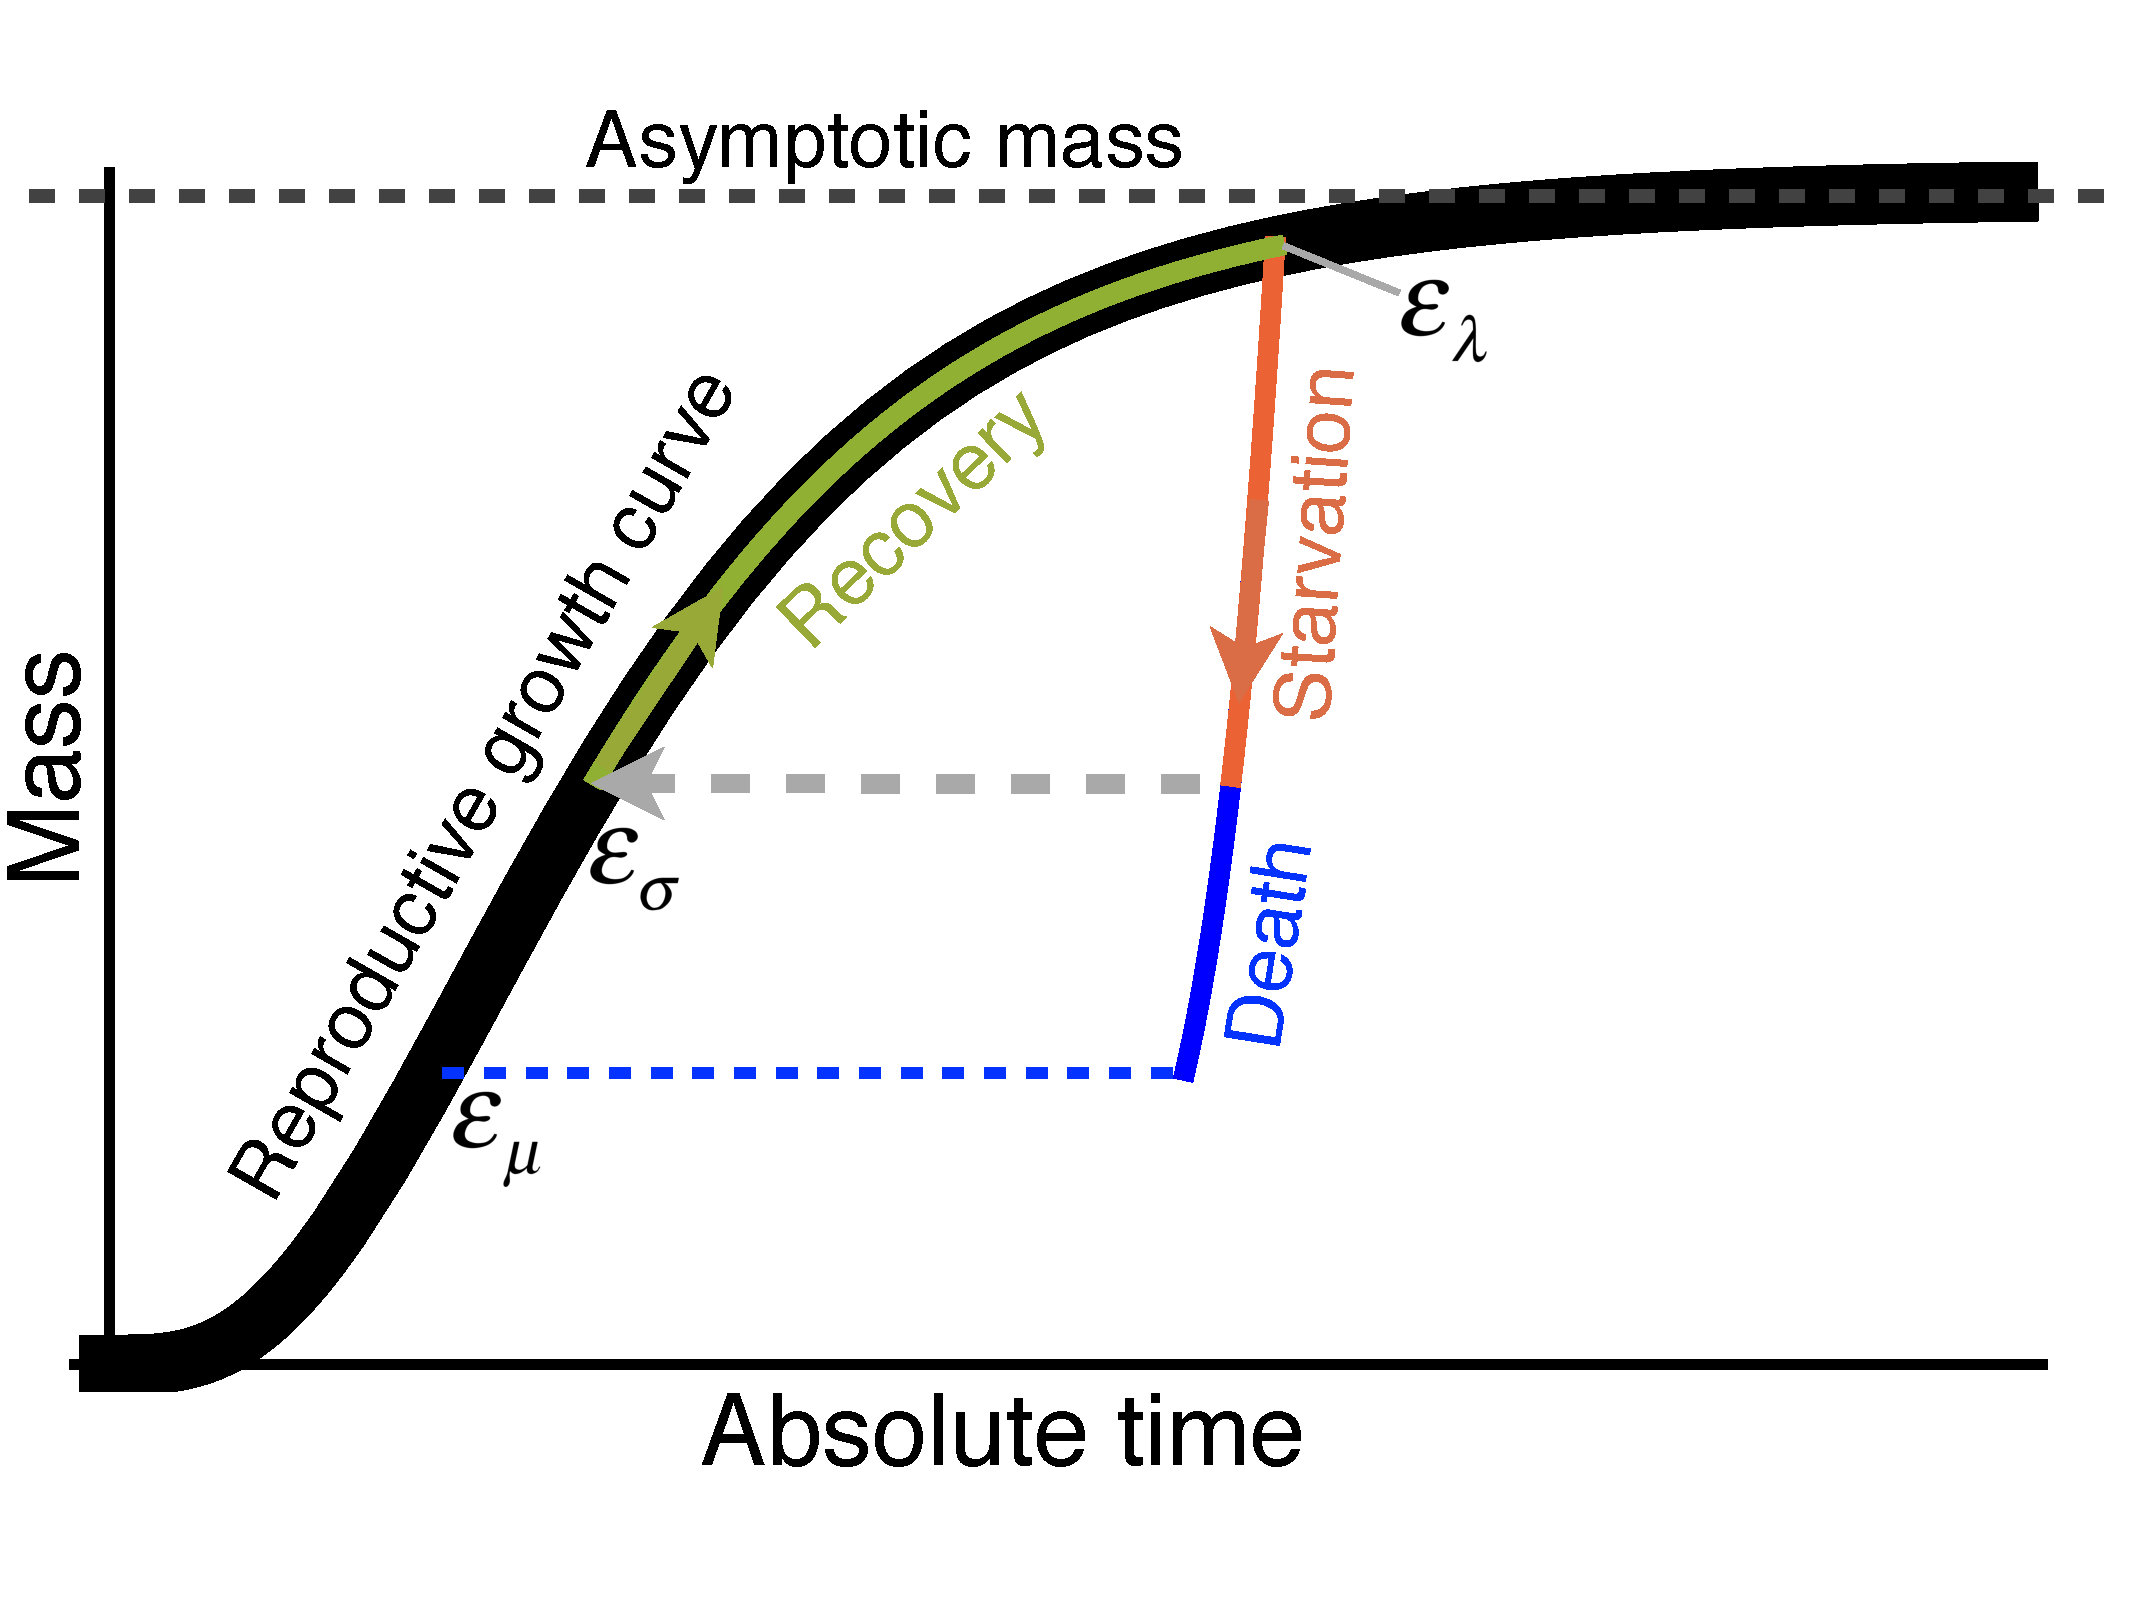
\includegraphics[width=0.5\textwidth]{Growth-trajectory-diagram.pdf}
\caption{ % 58 words
}
\label{fig:growth}
\end{figure*}

\begin{figure*}
\centering
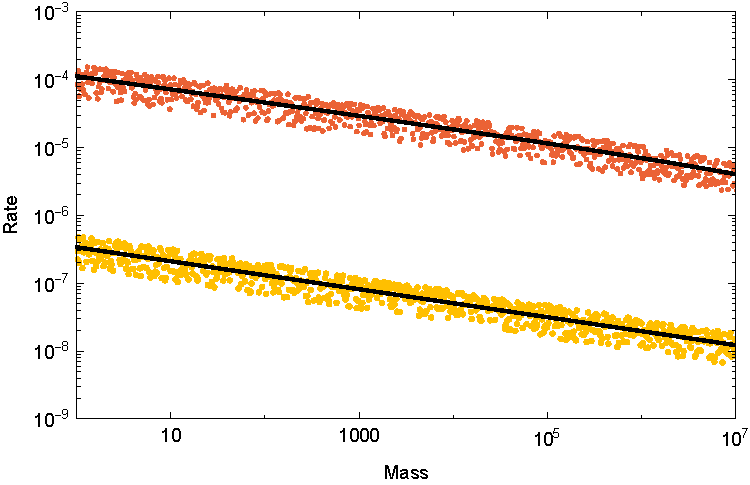
\includegraphics[width=0.5\textwidth]{fig_GvS.pdf}
\caption{ % 58 words
}
\label{fig:gvs}
\end{figure*}

\begin{figure*}
\centering
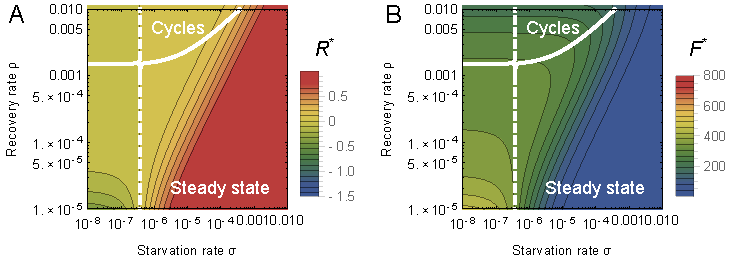
\includegraphics[width=0.5\textwidth]{fig_FixedPoint.pdf}
\caption{ % 58 words
}
\label{fig:fp}
\end{figure*}

\begin{figure*}
\centering
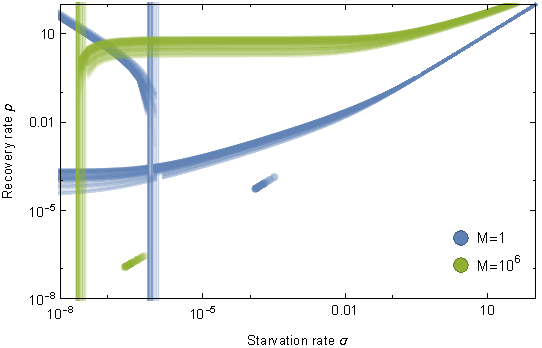
\includegraphics[width=0.5\textwidth]{fig_DataHopf.pdf}
\caption{ % 58 words
}
\label{fig:hopf}
\end{figure*}

\begin{figure*}
\centering
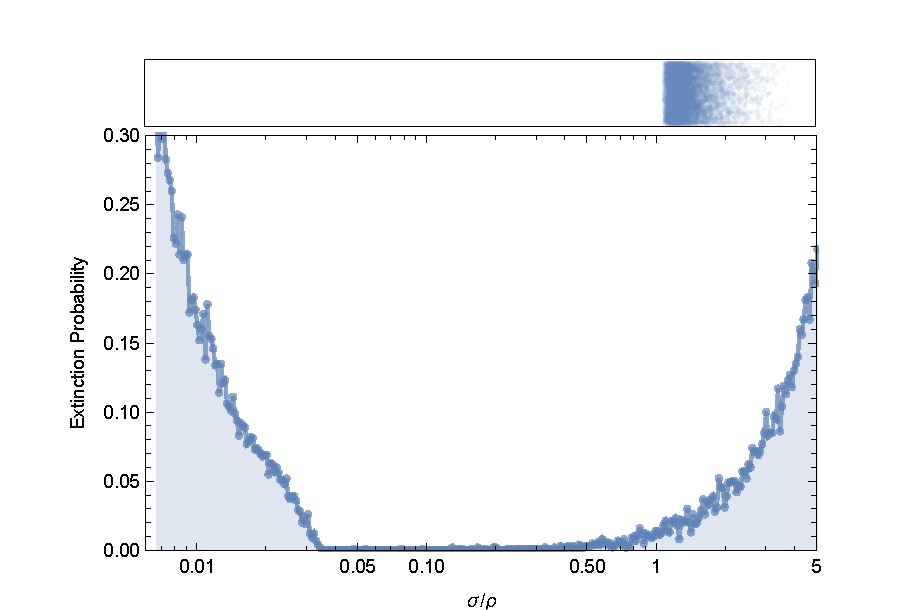
\includegraphics[width=0.5\textwidth]{fig_ExtinctionAllometric.pdf}
\caption{ % 58 words
}
\label{fig:ext}
\end{figure*} 
 
\begin{figure*}
\centering
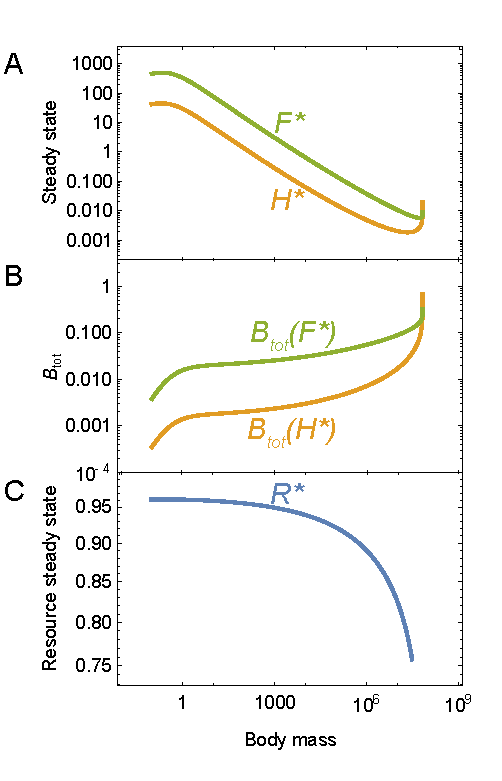
\includegraphics[width=0.45\textwidth]{fig_FPAllometric.pdf}
\caption{ % 58 words
}
\label{fig:mass}
\end{figure*}  
 
\begin{figure*}
\centering
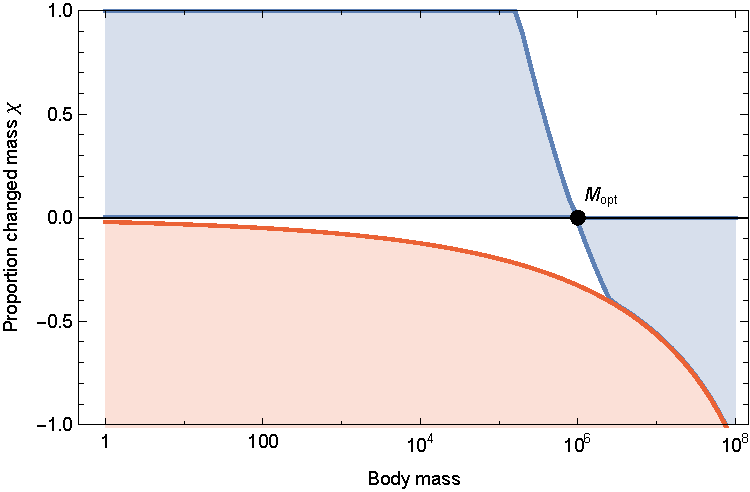
\includegraphics[width=1\textwidth]{fig_Invasion.pdf}
\caption{ % 58 words
}
\label{fig:invasion}
\end{figure*}  
 

% 
% 
%	 \begin{figure}[h]
%		 \centering
%		 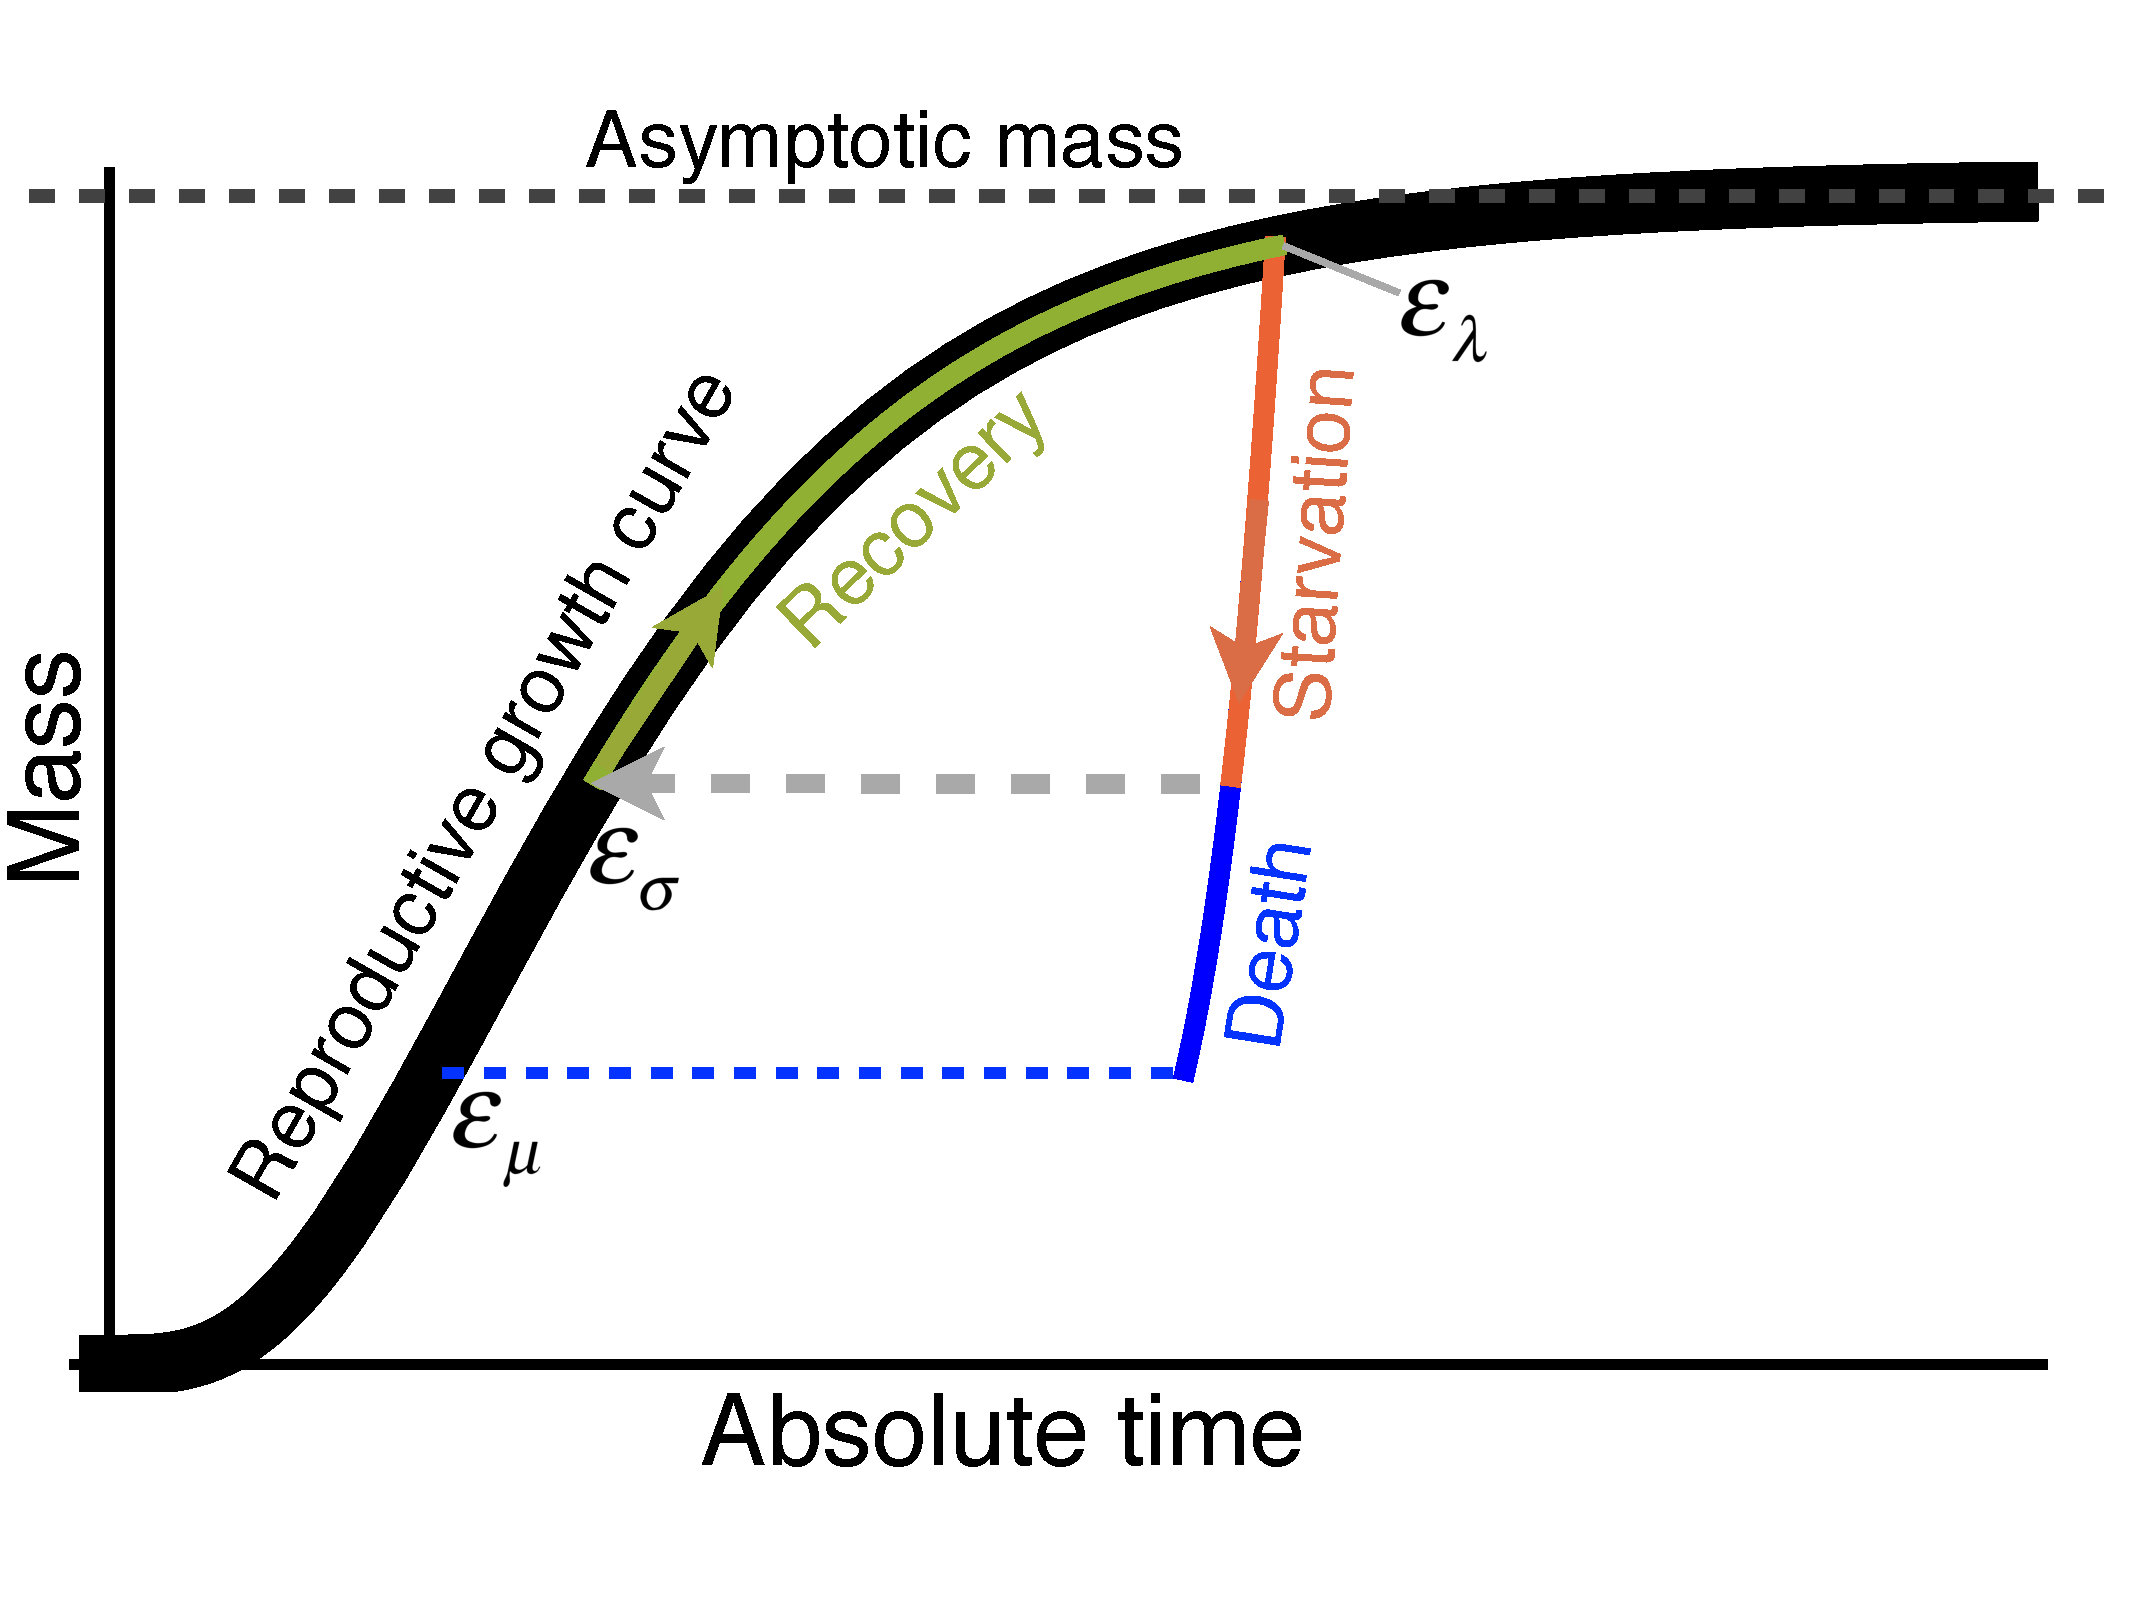
\includegraphics[width=0.5\textwidth]{Growth-trajectory-diagram.pdf}
%		 \caption{
%		 }
%		 \label{growth-diagram}
%	 \end{figure}
%	 
%	 \begin{figure}[h]
%		 \centering
%		 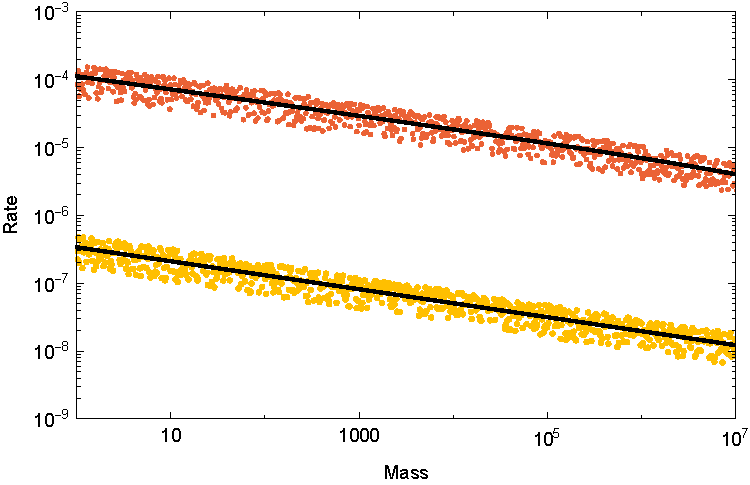
\includegraphics[width=0.25\textwidth]{fig_GvS.pdf}
%		 \caption{
%		 }
%		 \label{GvS}
%	 \end{figure}
%
%
%	\begin{figure}[h]
%	 	\centering
%	 	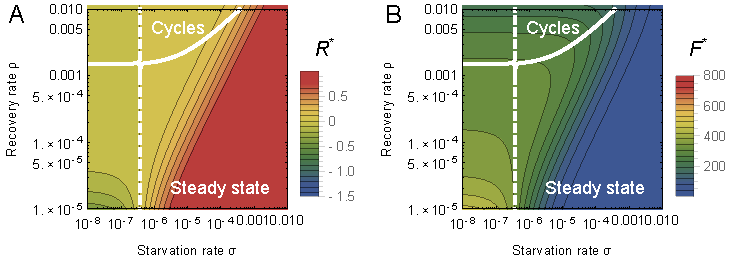
\includegraphics[width=0.25\textwidth]{fig_FixedPoint.pdf}
%	 	\caption{
%	 	}
%		\label{Hopfb}
%	\end{figure}
%
%
%	\begin{figure}[h]
%		\centering
%		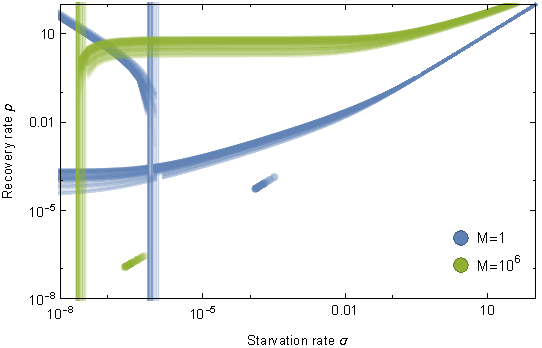
\includegraphics[width=0.8\textwidth]{fig_DataHopf.pdf}
%		\caption{
%		}
%		\label{DataHopf}
%	\end{figure}
%	 
% 
%	\begin{figure}[h]
%		\centering
%	 	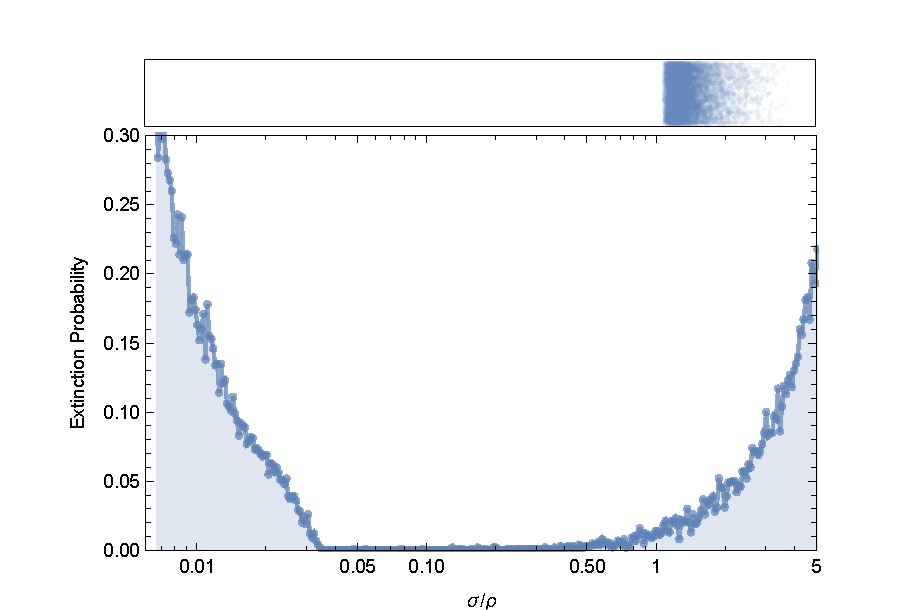
\includegraphics[width=0.8\textwidth]{fig_ExtinctionAllometric.pdf}
%	 	\caption{
%	 	}
%	 	\label{Ext}
%	\end{figure}
%	
%	\begin{figure}[h]
%	 	\centering
%	 	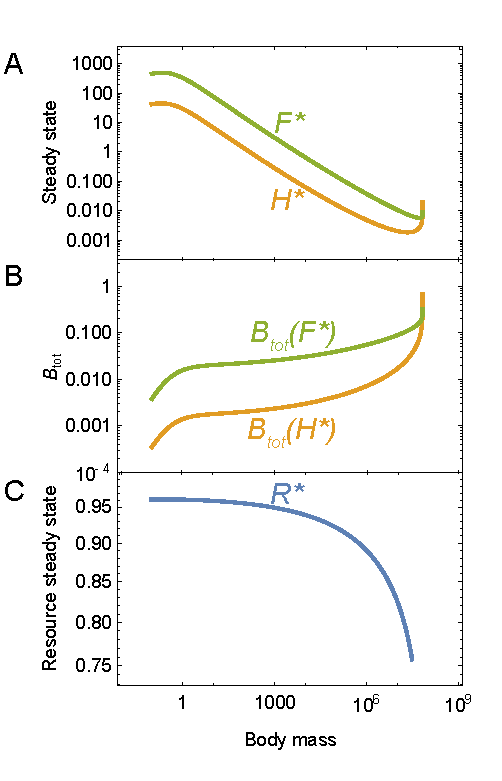
\includegraphics[width=0.5\textwidth]{fig_FPAllometric.pdf}
%	 	\caption{
%	 	}
%	 	\label{Asymp}
%	\end{figure}
%
\clearpage

\begin{table}[h]
\caption{Parameter Values For Various Classes of Organisms}
\label{param}
    \begin{center}
    \small
     \begin{tabular}{| p{1.2cm}| p{3.2cm} | p{2.6cm} | p{3.2cm} | }
     \hline
     & {\bf Mammals} & {\bf Unicellular Eukaryotes} & {\bf Bacteria} \\
     \hline
   $\eta$ & $3/4$ & & $1.70$ \\ 
   $E_{m}$ & $10695$ (J gram$^{-1}$) & & $10695$ (J gram$^{-1}$) \\ 
   $E_{m}^{\prime}$ & $\approx E_{m}$ & & $\approx E_{m}$ \\ 
   $B_{0}$ & $0.019$ (W gram$^{-\alpha}$) & & $1.96\times10^{17}$ \\
   $B_{m}$ & $0.025$ (W gram$^{-1}$)   & & $0.025$ (W gram$^{-1}$)\\
   $a$ & $1.78\times10^{-6}$ & & $1.83\times10^{13}$ \\ 
   $b$ & $2.29\times10^{-6}$ & & $2.29\times10^{-6}$ \\  
   $\eta-1$ & $-0.21$ & & $0.73$ \\ 
   $\lambda_{0}$ & $3.39\times10^{-7}$ (s$^{-1}$ gram$^{1-\eta}$) & & $56493$ \\ 
   $\gamma$ & $1.19$ & & $0.68$ \\ 
   $f_{0}$ & $0.02$ & & $1.30\times10^{-5}$ \\ 
   $\zeta$ & $1.01$ & & \\ 
   $mm_{0}$ & $0.32$ & & \\ 
   
      
   \hline
    \end{tabular}
    \end{center}
   \end{table}



\end{document}






















